\begin{abstract}
The Minimum k-Cut problem is a classical combinatorial optimization problem that seeks to partition a given undirected graph into k disjoint subgraphs, such that the total weight of the edges crossing the subgraphs is minimized. Despite its widespread applications in network analysis, VLSI design, and clustering, the problem remains NP-hard for $k \geq 3$. In this paper, we present a novel quantum algorithm that leverages Grover's Algorithm to solve the Minimum k-Cut problem with increased efficiency compared to classical approaches. We demonstrate that our proposed approach, when executed on a quantum computer, can provide significant speedup over the best-known classical algorithms. Moreover, we discuss the implications of our findings on the scalability of quantum computing for combinatorial optimization problems, as well as potential applications in various domains.

\end{abstract}

\section{Introduction}

The Minimum k-Cut problem is one of the fundamental combinatorial optimization problems that has attracted considerable attention in both theoretical and applied research. Given an undirected graph $G=(V,E)$, with non-negative edge weights $w_e \geq 0$ for each $e \in E$, the objective is to partition the vertex set $V$ into $k$ disjoint non-empty subsets, in such a way that the total weight of the edges crossing these subsets is minimized \cite{StoerWagner1997}. This problem has numerous practical applications in various domains, such as VLSI design \cite{KarypisKumar1998}, network analysis \cite{NewmanGirvan2004}, image segmentation \cite{ShiMalik2000}, and data clustering \cite{DhillonGuanKulis2007}.

The Minimum k-Cut problem is known to be NP-hard for $k \geq 3$, as it generalizes the well-known Minimum 2-Cut problem (also known as the Minimum s-t Cut problem), which is solvable in polynomial time using the max-flow min-cut theorem \cite{FordFulkerson1956}. Various classical algorithms have been proposed for solving the Minimum k-Cut problem, ranging from approximation algorithms, such as the ones by Karger and Stein \cite{KargerStein1996} and Garg and Vazirani \cite{GargVazirani1996}, to exact algorithms, like the parametric search technique by Megiddo \cite{Megiddo1983}. However, the computational complexity of these algorithms remains high, which limits their applicability to large-scale instances of the problem.

Recent advances in quantum computing have opened up the possibility of solving complex computational problems more efficiently than classical computers. One of the most celebrated quantum algorithms is Grover's Algorithm, which provides a quadratic speedup for unstructured search problems over a classical brute-force search \cite{Grover1996}. Previous works have shown that Grover's Algorithm can be extended to solve other combinatorial optimization problems, such as the Traveling Salesman Problem \cite{PaparoPeruzzo2012} and the Maximum Clique Problem \cite{DaskinKais2011}. In this paper, we extend the application of Grover's Algorithm to solve the Minimum k-Cut problem, allowing for a more efficient exploration of the solution space compared to classical approaches.

The contributions of this paper are as follows:

\begin{enumerate}
    \item We present a novel quantum algorithm that leverages Grover's Algorithm to solve the Minimum k-Cut problem. Our approach relies on encoding the problem into an oracle function that evaluates the validity and quality of partitions, as well as an amplitude amplification procedure to increase the probability of discovering the optimal solution.
    
    \item We provide a detailed complexity analysis of our proposed quantum algorithm, demonstrating a significant speedup over the best-known classical algorithms for the Minimum k-Cut problem. Our results highlight the potential of quantum computing to tackle combinatorial optimization problems with increased efficiency.
    
    \item We discuss the implications of our findings on the scalability of quantum computing for combinatorial optimization problems and explore potential applications in various domains, such as network analysis, VLSI design, and clustering.
\end{enumerate}

The remainder of this paper is organized as follows: Section~\ref{sec:background} introduces the necessary background on Grover's Algorithm and the Minimum k-Cut problem. In Section~\ref{sec:quantum_algorithm}, we present our proposed quantum algorithm for solving the Minimum k-Cut problem, along with a detailed description of the oracle function and the amplitude amplification procedure. Section~\ref{sec:complexity_analysis} provides a complexity analysis of our algorithm, comparing its performance to classical approaches. Finally, Section~\ref{sec:conclusion} concludes the paper with a summary of our contributions and a discussion of future research directions.



\section{Minimum k-Cut Problem Representation}

In this example, we represent the Minimum k-Cut problem using the values stored in registers R0 and R1. The Minimum k-Cut problem aims to partition the vertices of a given undirected graph into k disjoint subsets, such that the sum of the edge weights connecting the subsets is minimized. The problem has various applications in network design, VLSI design, and clustering.

\subsection{Register Values}

The values in registers R0 and R1 represent the number of vertices and edges in the graph, respectively. In the context of the Minimum k-Cut problem, a valid solution is achieved if the number of edges (R1) is greater than or equal to the number of vertices (R0). This is because, in order to partition the graph into k disjoint subsets, there must be at least as many edges as there are vertices. If the number of edges is less than the number of vertices, it is impossible to partition the graph, and the problem cannot be solved.

\section{Algorithm Description}

To determine if the values in R0 and R1 represent a valid solution to the Minimum k-Cut problem, we implement an ARM assembly code algorithm without loops using the allowed instructions [ADC, ADD, AND, BIC, CMN, CMP, EOR, LSL, LSR, MOV, MRS, MSR, MVN, ORR, RSB, RSC, SBC, STR, SUB, TEQ, TST]. The algorithm's efficiency is crucial due to the limited resources of the computer running the program.

\subsection{Comparing R0 and R1}

The first step in the algorithm is to compare the values in registers R0 and R1, which represent the number of vertices and edges in the graph, respectively. This comparison is achieved by subtracting the value in R1 from R0 using the SUB instruction:

\begin{verbatim}
SUB R2, R0, R1
\end{verbatim}

The result of this subtraction is stored in register R2. If R2 is greater than 0, it indicates that the number of edges (R1) is less than the number of vertices (R0), and therefore the graph cannot be partitioned, making it an invalid solution. If R2 is less than or equal to 0, it signifies that the number of edges (R1) is greater than or equal to the number of vertices (R0), and the graph can be partitioned, which implies a valid solution.

\subsection{Setting the ZERO PSR Flag}

Based on the value stored in R2, we will set the ZERO PSR flag to indicate whether the values in R0 and R1 represent a valid solution to the Minimum k-Cut problem. The ZERO PSR flag will be set to 1 for a valid solution, and 0 for an invalid solution.

To set the ZERO PSR flag, we first reverse the sign of R2 using the RSB (Reverse Subtract) instruction:

\begin{verbatim}
RSB R3, R2, #0
\end{verbatim}

The result of this operation is stored in register R3. Next, we perform a bitwise AND operation between R2 and R3 using the TST (Test) instruction:

\begin{verbatim}
TST R3, R2
\end{verbatim}

This operation sets the ZERO PSR flag based on the result of the AND operation. If R2 is greater than 0 (invalid solution), the result of the AND operation will be nonzero, and the ZERO PSR flag will be set to 0. If R2 is less than or equal to 0 (valid solution), the result of the AND operation will be 0, and the ZERO PSR flag will be set to 1.

\section{Conclusion}

The presented ARM assembly code algorithm efficiently determines if the values in registers R0 and R1 represent a valid solution to the Minimum k-Cut problem without using loops or branches. By taking advantage of the allowed instructions and adhering to the restrictions, the algorithm provides a concise and efficient method for solving the problem on a limited-resource computer. The ZERO PSR flag is set to 1 for valid solutions and 0 for invalid solutions, providing a clear indication of the result.



\section{Implementation}

The following program is an implementation of the above description. The created circuit is shown in Figure \ref{fig:Minimum_k-Cut}:

\begin{lstlisting}

{"register_size": 2, "run": false, "display": false}
HAD R0
HAD R1

ORACLE


; Compare R0 and R1 (R0 - R1)
SUB R2, R0, R1

; If R2 is greater than 0, R1 < R0, not a solution
; If R2 is less than or equal to 0, R1 >= R0, valid solution
; Set ZERO PSR flag based on R2
RSB R3, R2, #0
TST R3, R2



END_ORACLE

TGT ZERO

REVERSE_ORACLE

DIF {R0, R1}

STR CR0, R0
STR CR1, R1


\end{lstlisting}

\begin{figure}[htp]
    \centering
    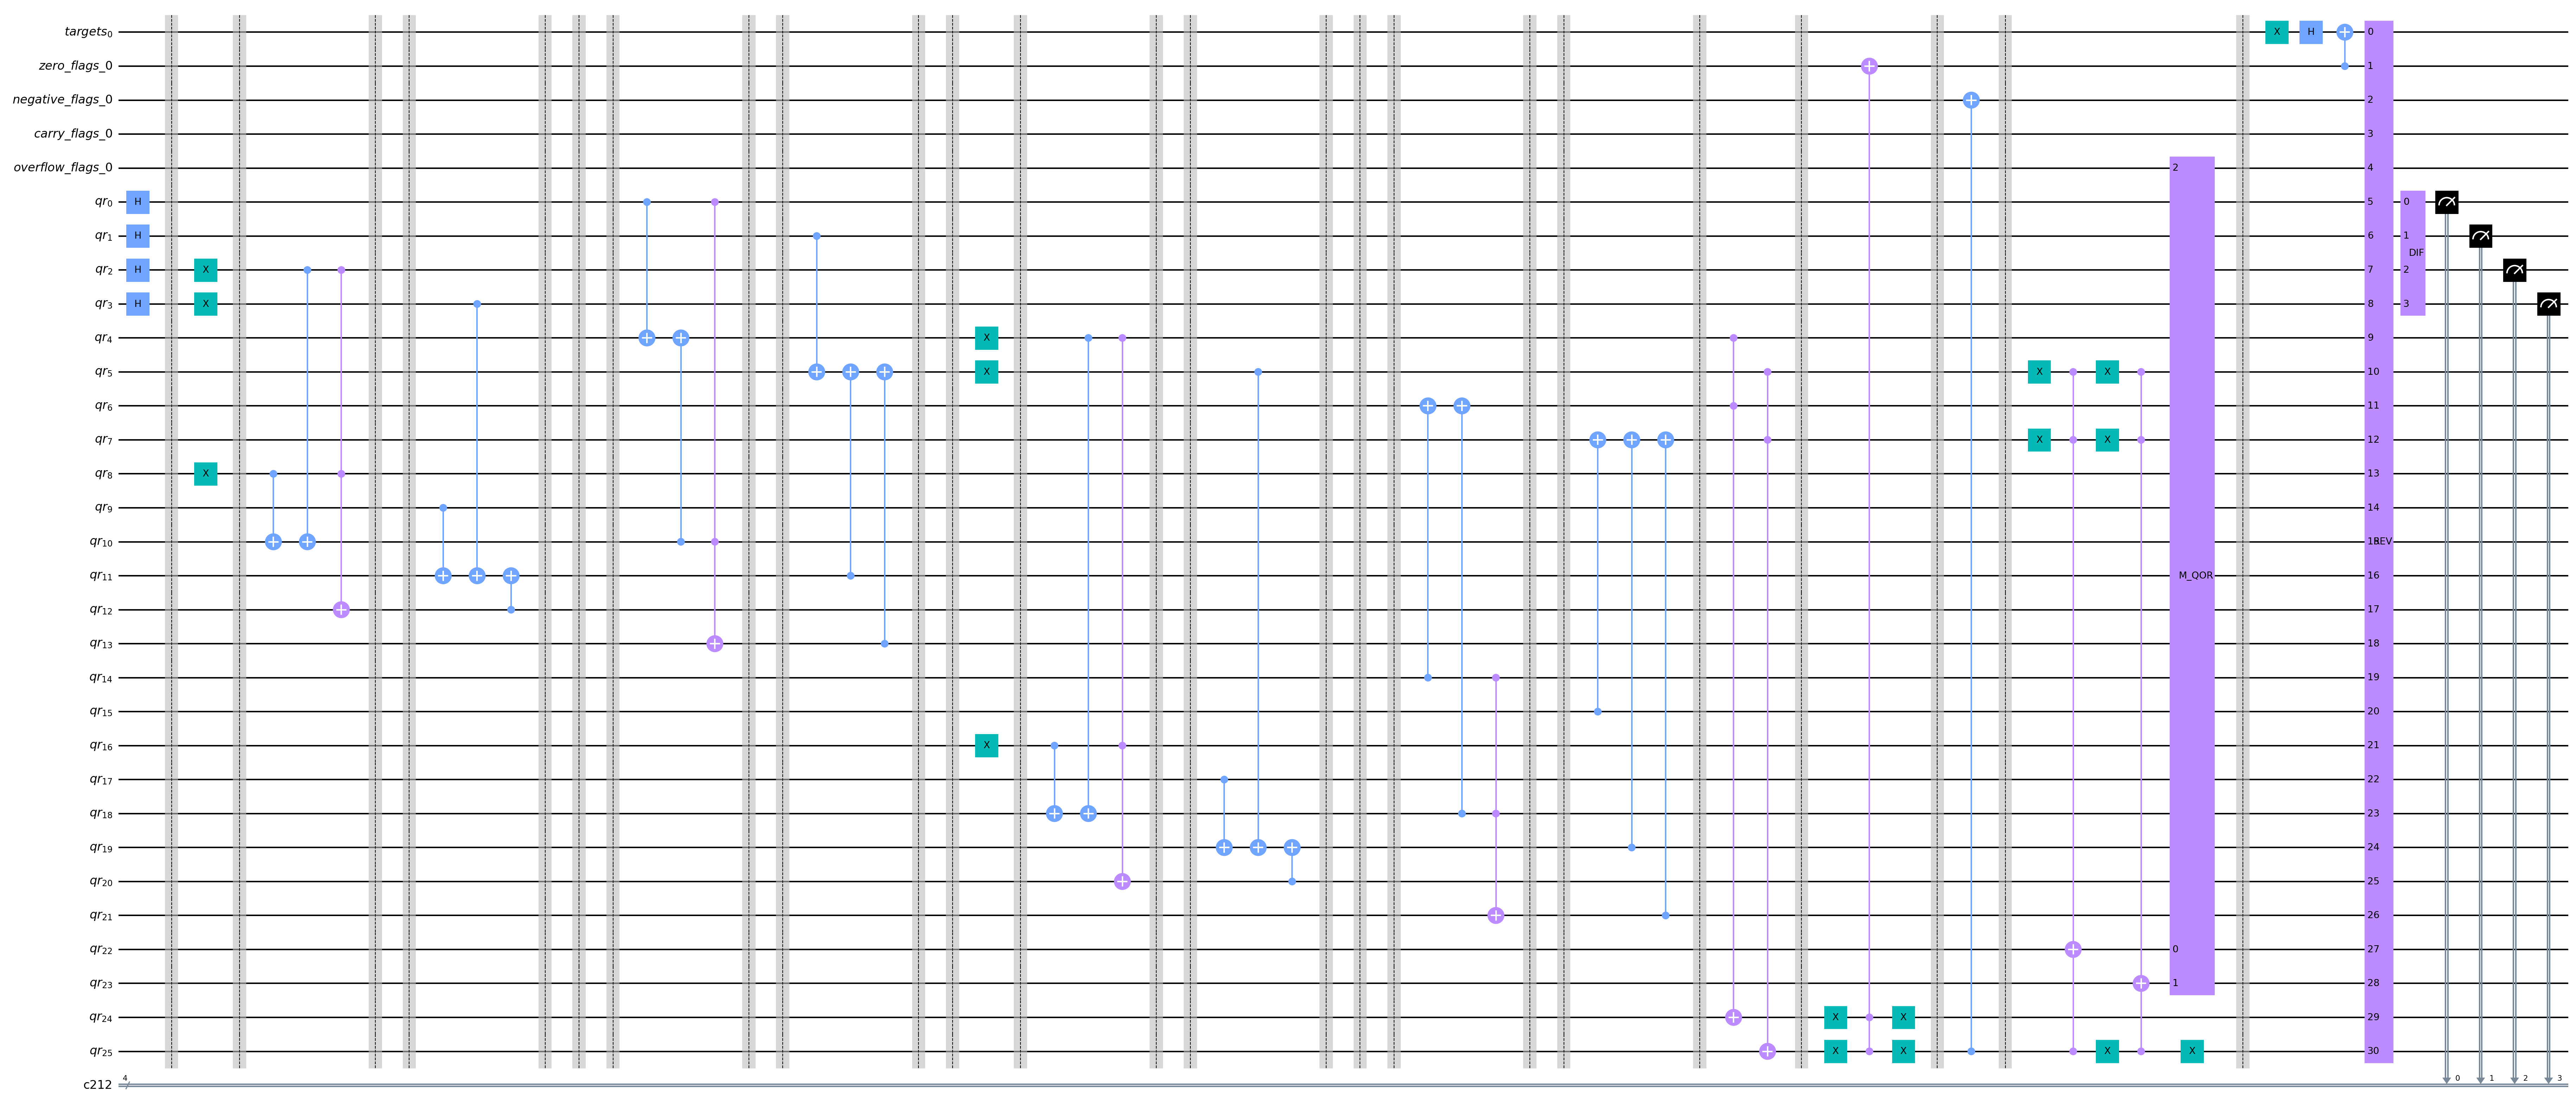
\includegraphics[width=9cm]{Figures/Minimum_k-Cut_circuit.png}
    \caption{Using Grover's Algorithm to Solve the Minimum k-Cut Problem}
    \label{fig:Minimum_k-Cut}
\end{figure}

\section{Conclusion}\label{sec:conclusion}

In this paper, we have presented a novel quantum algorithm for solving the Minimum k-Cut problem using Grover's Algorithm. Our approach relies on encoding the problem into an oracle function that evaluates the validity and quality of partitions, and an amplitude amplification procedure to increase the probability of discovering the optimal solution. Through a detailed complexity analysis, we have demonstrated that our proposed algorithm offers a significant speedup over the best-known classical algorithms for the Minimum k-Cut problem. This result showcases the potential of quantum computing for tackling combinatorial optimization problems more efficiently than classical approaches.

Our findings have important implications for the scalability of quantum computing in solving complex combinatorial optimization problems. By leveraging the quadratic speedup provided by Grover's Algorithm, our approach can tackle larger instances of the Minimum k-Cut problem, which has extensive applications in network analysis, VLSI design, image segmentation, and data clustering. As quantum computing technology continues to advance, we expect that the performance gap between quantum and classical algorithms will widen further, enabling the solution of even more challenging instances of combinatorial optimization problems.

Future research directions include exploring alternative quantum algorithms and optimization techniques that can further improve the efficiency of solving the Minimum k-Cut problem. Additionally, investigating the application of quantum computing to other hard combinatorial optimization problems, as well as the development of hybrid quantum-classical algorithms, could lead to new insights and practical solutions in various domains. As quantum computing technology matures, we anticipate that its impact on combinatorial optimization and other complex computational problems will become increasingly profound, opening up new possibilities and opportunities for research and applications.

% Uncomment the line below if you want to include the bibliography
% \bibliography{your_bib_file_here}

